\documentclass{article}

\usepackage{amsmath}
\usepackage{upgreek}
\usepackage{dsfont}
\usepackage{mdframed}
%margin package
\usepackage[margin=1in,includefoot]{geometry}
%graphics packages
\usepackage{graphicx}
\usepackage{float}
%pseudocode packages
\usepackage{amsmath}
\usepackage{algorithm}
\usepackage[noend]{algpseudocode}
\usepackage{listings}


\begin{document}

\begin{enumerate}

%% PROBLEMA 6 %%%%%%%%%%%%%%%%%%%%%%%%%%%%%%%%%%%%%%%%%%%%%%%%%%%%%%%%%%%%%%%%%%

% Enunciado %%%%
\item Asumiendo que la factorizaci\'on LU de la matriz A existe, probar que :
\begin{itemize}
%% PART a) -----------------------
\item $A$ puede ser escrita en la forma :

\begin{gather*}
A = L D U_{1}
\end{gather*}
donde $D$ es una matriz diagonal, y $L$ y $U_{1}$ son matrices triangulares unitarias ( con $1$ en la diagonal principal ) inferior y superior respectivamente.\\

%% Solución %%%%

Empecemos por escribir $A$ como su factorizaci\'on $LU$, y de ahí procedamos a formar la factorizaci\'on $LDU_{1}$, como sigue : \\

Tenemos
\begin{gather*}
A = LU, U = 
\begin{bmatrix}
	u_{11}  & u_{12} & \hdots & u_{1n} \\
	   0    & u_{22} \\
	 \vdots && \ddots \\
	   0    & \hdots && u_{nn}
\end{bmatrix}
\end{gather*}
Y queremos expresarlo en la forma
\begin{gather*}
A = LDQ,\textit{ } D = 
	\begin{bmatrix}
		d_{11}  & 	0	 & \hdots & 0 \\
		   0    & d_{22} \\
		 \vdots && \ddots \\
		   0    & \hdots && d_{nn}		   
	\end{bmatrix}
Q = 
	\begin{bmatrix}
		   1    & q_{12} & \hdots & q_{1n} \\
		   0    &    1    \\
		 \vdots && \ddots \\
		   0    & \hdots && 1
	\end{bmatrix}
\end{gather*}

Bastaría con poder probar que podemos expresar $U$ como $U = DQ$, para lo cu\'al analizaremos el elemento $u_{ij}$ de $U$ para poder sacar una correspondencia con los elementos $d_{ij}$ y $q_{ij}$ de las otras matrices. Si llegamos a poder expresar todo $u_{ij}$ en funci\'on de $d_{ij}$ y $q_{ij}$ entonces tendremos que podemos expresar la matriz $U$ en funci\'on de $D$ y $Q$. Procedamos entonces comparando los t\'erminos, as\'i :

\begin{gather*}
D_{ij} = 
	\begin{cases}
		0,	& i \neq j \\
		d_{ii},	& i = j
	\end{cases},
Q_{ij} = 
	\begin{cases}
		q_{ij},	& i < j \\
		1	  ,	& i = j \\
		0	  ,	& i > j
	\end{cases}, \rightarrow 
DQ_{ij} = 
	\begin{cases}
		d_{ii} * q_{ij}	,	& i < j \\
		d_{ii}			,	& i = j \\
		0	  			,	& i > j
	\end{cases}\\
U_{ij} = 
	\begin{cases}
		u_{ij},	& i < j \\
		u_{ii},	& i = j \\
		0	  ,	& i > j	
	\end{cases}
\end{gather*}

De comparar las reglas de correspondencia para cada $i,j$ en los rangos dados, tenemos que :

\begin{gather*}
u_{ii} = d_{ii}, i = j\\
u_{ij} = d_{ii}q_{ij}, i < j \\
\rightarrow 
D_{ij} = 
	\begin{cases}
		0	  ,	& i \neq j \\
		u_{ii},	& i = j
	\end{cases},
Q_{ij} = 
	\begin{cases}
		\frac{u_{ij}}{u_{ii}} ,	& i < j \\
		1	  				  ,	& i = j \\
		0	  				  ,	& i > j
	\end{cases} 
\end{gather*}

Por lo que si la factorizaci\'on $A=LU$ existe, podemos expresar $A$ como $A=LDQ$, siendo $D$ y $Q$ matrices diagonal y triangular superior-unitaria con elementos en funci\'on de la matrix $U$ seg\'un la f\'ormula anterior.

%% PART b) -----------------------

% Enunciado %%%%
\item Si $A$ es sim\'etrica, entonces :
\begin{gather*}
A = LDL^{T}
\end{gather*}

%% Solución %%%%
Si $A$ es sim\'etrica, entonces $A=A^{T}$. Reemplazando la factorizaci\'on anterior y usando las propiedades de la transpuesta tenemos :

\begin{gather*}
A = LDU \rightarrow A^{T} = (LDU)^{T} = U^{T}D^{T}L^{T} = U^{T}DL^{T} \\
\rightarrow LDU = U^{T}DL^{T}
\end{gather*}

De lo anterior, podemos observar que la igualdad se cumple si tenemos que $U=L^{T}$, ya que tendr\'iamos que :
\begin{gather*}
A = LDU = LD(L^{T}) = A^{T} = U^{T}DL^{T} = (L)DL^{T}
\end{gather*}

Para probar esto, procederemos a usar inducci\'on de la siguiente forma :

\begin{itemize}
\item El caso base es f\'acil de probar, usando $k = 2$, para lo cu\'al usamos: 
\begin{gather*}
U = 
\begin{bmatrix}
	1  & u_{12} \\
	0  &   1
\end{bmatrix}, 
L = 
\begin{bmatrix}
	   1    &   0    \\
	l_{21}  &   1
\end{bmatrix}\\
\rightarrow
U^{T}DL^{T} = 
\begin{bmatrix}
	   d_{11}     &   d_{11}u_{12}    \\
	d_{11}l_{21}  &   d_{22} + d_{11}l_{21}u_{12}
\end{bmatrix}\\
\rightarrow
LDU = 
\begin{bmatrix}
	   d_{11}     &   d_{11}l_{21}    \\
	d_{11}u_{12}  &   d_{22} + d_{11}l_{21}u_{12}
\end{bmatrix}
\end{gather*}

Igualando, tenemos que $l_{21} = u_{12}$, por lo que $U = L^{T}$, lo cu\'al prueba el caso base.\\

\item Asumamos que para un orden $k = n$ se cumple lo siguiente :
\begin{gather*}
U^{T}DL^{T} = LDU \rightarrow U = L^{T}
\end{gather*}
Usaremos esto para probar el caso $k = n+1$.\\

\item Probemos que para $k = n + 1$ se cumple $U'^{T}D'L'^{T} = L'D'U' \rightarrow U' = L'^{T}$. Para esto, formemos la matrices de la siguiente forma :

\begin{gather*}
U'^{T}D'L'^{T} = 
\begin{bmatrix}
	U^{T}_{nxn}  & \theta_{n+1,1} \\
	 u^{T}_{n+1} & 1
\end{bmatrix}
	\begin{bmatrix}
		D_{nxn} & 0 \\
		   0    & d_{n+1}
	\end{bmatrix}
		\begin{bmatrix}
			L^{T}_{nxn}  	   & l^{T}_{n+1} \\
			    \theta_{1,n+1} & 1
		\end{bmatrix}
\\
L'D'U' = 
\begin{bmatrix}
	L_{nxn}  & \theta_{n+1,1} \\
	 l_{n+1} & 1
\end{bmatrix}
	\begin{bmatrix}
		D_{nxn} & 0 \\
		   0    & d_{n+1}
	\end{bmatrix}
		\begin{bmatrix}
			U _{nxn}  	& u_{n+1} \\
		 \theta_{1,n+1} & 1
		\end{bmatrix}
\end{gather*}

Si reducimos operando por bloques, tenemos :

\begin{gather*}
U'^{T}D'L'^{T} =
\begin{bmatrix}
	U^{T}DL^{T}  		 & U^{T}Dl^{T}_{n+1} \\
	 (du)^{T}_{n+1}L^{T} & d_{n+1} + <(du)^{T}_{n+1}, l^{T}_{n+1}>
\end{bmatrix}
\\
LDU =
\begin{bmatrix}
			DLU  		 & LDu_{n+1} \\
	 (dl)_{n+1}U 		 & d_{n+1} + <(dl)_{n+1},u_{n+1}>
\end{bmatrix}
\end{gather*}

Si comparamos, tenemos que para el bloque de $nxn$, aplicando la suposici\'on que se hizo por inducci\'on :

\begin{gather*}
U'^{T}D'L'^{T} = LDU \rightarrow U_{nn} = L^{T}_{nn}
\end{gather*}

Comparando el resto de las 2 matrices de $n+1,n+1$ tenemos que :
\begin{gather*}
U^{t}Dl^{T}_{n+1} = LDu_{n+1} \rightarrow LDl^{T}_{n+1} = LDu_{n+1}\\
\rightarrow
LD(l^{T}_{n+1} - u_{n+1}) = \theta \rightarrow u_{n+1} = l^{T}_{n+1} \\
\rightarrow u_{q,n+1} = l_{n+1,q}, \forall q=1,\hdots,n
\end{gather*}

Los cu\'ales eran los elementos restantes de las matrices $L',U'$. Dado que obtuvimos $U_{nxn} = L^{T}_{nxn}$, y que $u_{q,n+1} = l_{n+1,q}, \forall q=1,\hdots,n$, tenemos que las matrices $L'_{n+1xn+1}, U'_{n+1xn+1}$ cumplen :

\begin{gather*}
U'_{n+1xn+1} = L'^{T}_{n+1xn+1}
\end{gather*}

Lo cu\'al completa la prueba por inducci\'on, lo que nos permite concluir que :

\begin{gather*}
If : A=A^{T} \rightarrow A=LDL^{T}
\end{gather*}

%% PART c) -----------------------


% Enunciado %%%%%%%
\item Si $A$ es sim\'etrica y definida positiva, entonces :
\begin{gather*}
A=HH^{T}
\end{gather*} %%%%%
Donde H es una matriz triangular inferior con elementos positivos en la diagonal principal ( descomposici\'on de Cholesky )\\
%% Solución

Empecemos de la factorizaci\'on anterior, ya que $A$ es sim\'etrica.

\begin{gather*}
A = LDL^{T}
\end{gather*}

Dado que $A$ es definida positiva, tenemos que :
\begin{gather*}
q^{T}Aq > 0 \forall q, \rightarrow q^{T}LDL^{T}q = (L^{T}q)^{T}D(L^{T}q) > 0 \forall q
\end{gather*}

Haciendo $r = L^{T}q$ tenemos que:

\begin{gather*}
r^{T}Dr > 0 \forall r \rightarrow d_{1}r^{2}_{1} + \hdots + d_{n}r^{2}_{n} > 0 \forall r_{i},d_{i}\\
\rightarrow d_{i} > 0 \forall i=1,\hdots,n
\end{gather*}

Obtenemos entonces que la matriz $D$ debe tener elementos positivos en la diagonal principal, lo cu\'al nos permite separar a la matriz $D$ en $D^{1/2}D^{1/2}$, siendo :

\begin{gather*}
D^{1/2}_{ij} = 
	\begin{cases}
			0 		 , i \neq j\\
		\sqrt{d_{i}} , i=j
	\end{cases}
\end{gather*}

Con esto, podemos expresar $A$ de la siguiente manera :

\begin{gather*}
A = LD^{1/2}D^{1/2}L^{T} = LD^{1/2}( D^{1/2} )^{T}L^{T} = (LD^{1/2})(LD^{1/2})^{T} \\
\rightarrow A = HH^{T},H= LD^{1/2}
\end{gather*}

Lo cu\'al comprueba el enunciado.

\end{itemize}

\end{itemize}

%% PROBLEMA 26 %%%%%%%%%%%%%%%%%%%%%%%%%%%%%%%%%%%%%%%%%%%%%%%%%%%%%%%%%%%%%%%%%

%% Enunciado %%%%%%%%%
\item Considere el sistema sim\'etrico $Ax=b$, donde :
\begin{gather*}
A = 
	\begin{bmatrix}
		0.4445 &  0.4444 & -0.2222\\
		0.4444 &  0.4445 & -0.2222\\
	   -0.2222 & -0.2222 &  0.1112
	\end{bmatrix},
b = 
	\begin{bmatrix}
		0.6667 \\
		0.6667 \\
	   -0.3332
	\end{bmatrix}
\end{gather*}
La soluci\'on exacta al sistema es:
\begin{gather*}
x = 
	\begin{bmatrix}
		1\\1\\1
	\end{bmatrix}
\end{gather*}

\begin{itemize}
%% Part a) --------
\item Aplique una perturbaci\'on $\delta b$ en $b$, manteniendo $A$ sin alterar. Resuelva el sistema $Ax' = b + \delta b$. Compare $x'$ con $x$. Calcule $Cond(A)$ y verifique la desigualdad respectiva para una perturbaci\'on en $b$.
\\
Sea :
\begin{gather*}
\delta b = 
	\begin{bmatrix} 
		0.0001 \\
		0.0001 \\
		0.0001 
	\end{bmatrix}
\Rightarrow
b' = 
	\begin{bmatrix}
		 0.6668 \\
		 0.6668 \\
		-0.3331
	\end{bmatrix}
\end{gather*}
\\
Resolviendo el sistema perturbado $Ax'=b'$ tenemos que :
\begin{gather*}
x' = 
	\begin{bmatrix}
		1.3334 \\
		1.3334 \\
		2.3333
	\end{bmatrix}
\rightarrow 
\delta x = 
	\begin{bmatrix}
		0.3334 \\
		0.3334 \\
		1.3333
	\end{bmatrix}
\end{gather*}
\\
Calculando el error relativo tenemos que, usando la norma 
$\Vert \textit{ } \Vert_{\infty}$ :

\begin{gather*}
\Vert x \Vert_{\infty} = 1,\textit{ }
\Vert \delta x \Vert_{\infty} = 1.3333 \\
\Vert \delta b \Vert_{\infty} = 0.0001,\textit{ }
\Vert  b \Vert_{\infty} = 0.6667 \\
\Vert  A \Vert_{\infty} = 1.1111,\textit{ }
\Vert  A^{-1} \Vert_{\infty} = 13333 \rightarrow Cond(A) = 14814.2963
\end{gather*}

Con lo anterior podemos confirmar que la siguiente desigualdad se cumple :

\begin{gather*}
\frac{ \Vert \delta x \Vert_{\infty} }{\Vert x \Vert_{\infty}} = 1.3333 \\
Cond(A) \frac{ \Vert \delta b \Vert_{\infty} }{ \Vert b \Vert_{\infty} } = 2.22 \geq 1.3333 \\
\rightarrow 
	\frac{ \Vert \delta x \Vert_{\infty} }{\Vert x \Vert_{\infty}} 
	\leq 
	Cond(A) \frac{ \Vert \delta b \Vert_{\infty} }{ \Vert b \Vert_{\infty} }
\end{gather*}

Con lo cu\'al vemos que se satisface la desigualdad para este caso.

%% Part b) --------
\item Aplique una pequeña perturbaci\'on $\Delta A$ en $A$ tal que 
$ \Vert \Delta A \Vert \leq 1 / \Vert A^{-1} \Vert $. Resuelva el sistema 
$ ( A + \Delta A ) x' = b $. Compare $x'$ con $x$ y verifique la desigualdad apropiada respecto a una perturbaci\'on en la matriz $A$ y el n\'umero condicionante.\\
%% Solución
\\
Elijamos una perturbaci\'on que satisfaga las condiciones. Para esto, escogemos :
\begin{gather*}
\Delta A = 
	\begin{bmatrix}
		0 & 0 & 0 \\
		0 & 0 & 0 \\
		1 & 0 & 0
	\end{bmatrix}  5 x 10^{-5}
\end{gather*}

Resolviendo el sistema $A'x' = b$ tenemos que :
\begin{gather*}
x' = 
	\begin{bmatrix}
		1.125 \\
		1.125 \\
		1.500
	\end{bmatrix}
\rightarrow
\delta x = 
	\begin{bmatrix}
		0.125 \\
		0.125 \\
		0.500
	\end{bmatrix}
\end{gather*}

Calculando las normas necesarias usando $\Vert \textit{ } \Vert_{\infty}$ tenemos que :
\begin{gather*}
\Vert x \Vert_{\infty} = 1,\textit{ }
\Vert \delta x \Vert_{\infty} = 0.5 \\
\Vert  \Delta A \Vert_{\infty} = 1.1111,\textit{ }
\end{gather*}

Usando estas normas, podemos comprar que se verifica la desigualdad correspondiente a una perturbaci\'on y el n\'umero condicionante :
\begin{gather*}
\frac{ \Vert \delta x \Vert_{\infty} }{\Vert x \Vert_{\infty}} = 0.5 \\
Cond(A) \frac{ \Vert \Delta A \Vert_{\infty} }{ \Vert A \Vert_{\infty} } /
( 1 - Cond(A) \frac{ \Vert \Delta A \Vert_{\infty} }{ \Vert A \Vert_{\infty} } 	) =  2.0 \\
\rightarrow 
\frac{ \Vert \delta x \Vert_{\infty} }{\Vert x \Vert_{\infty}}
\leq
Cond(A) \frac{ \Vert \Delta A \Vert_{\infty} }{ \Vert A \Vert_{\infty} } /
( 1 - Cond(A) \frac{ \Vert \Delta A \Vert_{\infty} }{ \Vert A \Vert_{\infty} } 	)\\
\end{gather*}
Con lo cu\'al comprobamos que se satisface la desigualdad correspondiente para este caso.
\\
\end{itemize}
%% PROBLEMA 5 %%%%%%%%%%%%%%%%%%%%%%%%%%%%%%%%%%%%%%%%%%%%%%%%%%%%%%%%%%%%%%%%%%
%% Enunciado
\item Implemente un programa que realice la descomposi\'on de Cholesky
\\
\\
%% Solución
Para esta descomposici\'on, usando la regla de correspondencia luego de igualar 
$A = LL^{T}$ tenemos que se cumple la siguiente relaci\'on :

\begin{gather*}
L_{jj} = \sqrt{ A_{jj} - \sum_{k=1}^{j-1} L_{jk}^{2} } \\
L_{ij} = \frac{1}{L_{jj}}( A_{ij} - \sum_{k=1}^{j-1} L_{ik}L_{kj} ), i>j
\end{gather*}
Usando esta relaci\'on podemos implementar el siguiente algoritmo en $c++$.
\\
\\
\\
\\
\\
\\
\\
\\
\\
\\
\\
\\
\\
\lstset{language=C++}
\begin{lstlisting}[frame=single]
namespace NLA {
  namespace decompositions {
    namespace lu {
        arma::mat cholesky( const mat &A )
        {
            assert( A.n_cols == A.n_rows );

            int N = A.n_cols;

            arma::mat _H = arma::zeros<mat>( N, N );

            for ( int p = 0; p < N; p++ )
            {
                double _sum = 0;
                for ( int k = 0; k <= p - 1; k++ )
                {
                    _sum += ( _H( p, k ) * _H( p, k ) );
                }
                _H( p, p ) = sqrt( A( p, p ) - _sum );

                for ( int q = p + 1; q < N; q++ )
                {
                    double _sum = 0;
                    for ( int k = 0; k <= p - 1; k++ )
                    {
                        _sum += ( _H( q, k ) * _H( p, k ) );
                    }
                    _H( q, p ) = ( A( q, p ) - _sum ) / _H( p, p );
                }
            }

            return _H;
        }
    }
  }
}
\end{lstlisting}
Estamos usando la librer\'ia $Armadillo$ para poder manejar matrices y no tener que crear nuestras propias clases para trabajar con matrices y vectores.

A continuaci\'on se muestra una prueba con una matriz definida positiva, usando nuestra implementaci\'on y compar\'andola con el resultado que se obtiene al usar la factorizaci\'on por defecto que usa la librer\'ia $Armadillo$.

\begin{figure}[H]
	\centering
	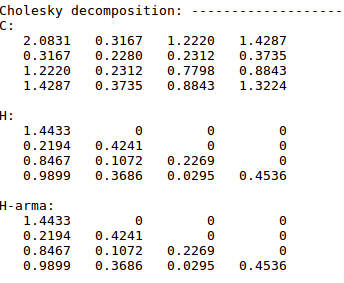
\includegraphics[scale=0.75]{/home/wilsan/Documents/wilbert/cs_master/courses/term1/numerical_linear_algebra/repo/hw/imgs/cholesky_test.png}
	\caption{Probando nuestra implementaci\'on de la descomposici\'onn de Cholesky}
	\label{fig:img_pecc}
\end{figure}

%% PROBLEMA 11 %%%%%%%%%%%%%%%%%%%%%%%%%%%%%%%%%%%%%%%%%%%%%%%%%%%%%%%%%%%%%%%%%


%%%%%%%%%%%%%%%%%%%%%%%%%%%%%%%%%%%%%%%%%%%%%%%%%%%%%%%%%%%%%%%%%%%%%%%%%%%%%%%%

\end{enumerate}



\end{document}